\documentclass[
	%parspace, % Térköz bekezdések közé / Add vertical space between paragraphs
	%noindent, % Bekezdésének első sora ne legyen behúzva / No indentation of first lines in each paragraph
	%nohyp, % Szavak sorvégi elválasztásának tiltása / No hypenation of words
	%twoside, % Kétoldalas nyomtatás / Double sided format
	%final, % Teendők elrejtése / Set final to hide todos
]{elteikthesis}[2019/06/10]
\usepackage{tikz}
\usepackage{xcolor}
\usepackage{pgfplots}

\definecolor{bblue}{HTML}{4F81BD}
\definecolor{rred}{HTML}{C0504D}
\definecolor{ggreen}{HTML}{9BBB59}
\definecolor{ppurple}{HTML}{9F4C7C}

% Dolgozat metaadatai
% Document's metadata
\title{Automatikus zenei hangszerfelismerés többszólamú zenében mély neuronhálók segítségével} % cím / title
\date{2020} % védés éve / year of defense

% Szerző metaadatai
% Author's metadata
\author{Hamrák János}
\degree{programtervező informatikus MSc}

% Témavezető(k) metaadatai
% Superivsor(s)' metadata
\supervisor{Gombos Gergő} % belső témavezető neve / internal supervisor's name
\affiliation{Adjunktus, PhD} % belső témavezető beosztása / internal supervisor's affiliation
%\extsupervisor{Külső Kornél} % külső témavezető neve / external supervisor's name
%\extaffiliation{informatikai igazgató} % külső témavezető beosztása / external supervisor's affiliation

% Egyetem metaadatai
% University's metadata
\university{Eötvös Loránd Tudományegyetem} % egyetem neve / university's name
\faculty{Informatikai Kar} % kar neve / faculty's name
\department{Programozáselmélet és Szoftvertechnológiai\\ Tanszék} % tanszék neve / department's name
\city{Budapest} % város / city
\logo{elte_cimer_szines} % logo

% Irodalomjegyzék hozzáadása
% Add bibliography file
\addbibresource{thesis.bib}

% A dolgozat
% The document
\begin{document}
	
% Nyelv kiválasztása
% Set document language
\documentlang{magyar}
%\documentlang{english}


% Dokumentum beállítások
% Some document settings
\input{settings.tex}

% Címlap (kötelező)
% Title page (mandatory)
\maketitle
\topicdeclaration

% Tartalomjegyzék (kötelező)
% Table of contents (mandatory)
\tableofcontents
\cleardoublepage

% Tartalom
% Main content
\chapter{Bevezetés} % Introduction
\label{ch:intro}

\section{Motiváció}
miért fontos, miért hasznos

\section{A dolgozat felépítése}

fejezetek kifejtése pár mondatban


\section{Kapcsolódó munkák}

Cite author  \citeauthor{li2015automatic} and cite \cite{han2016deep}. 
\cleardoublepage

\chapter{Elméleti háttér} 
\label{ch:theory}

Ebben a fejezetben a dolgozathoz kapcsolódó fogalmakat és elméleti alapokat mutatom be. Először magának a zenének a releváns tulajdonságairól ejtek szót. Ezután ismertetem a MIR kutatási területet, amelybe dolgozatom is tartozik. Majd végül a mesterséges intelligencián alapuló megoldásokról nyújtok elméleti bevezetőt, érintve a hagyományos gépi tanulás és a mély tanulás módszereit is.

\section{Zene és reprezentációi} 

\subsection{Zene fogalma, tulajdonságai}

A zene egy meglehetősen összetett fogalom. Az ember számára a zene megjelenhet például hang formájában, leírhatjuk őket szimbólumok segítségével egy kottában, előfordulhat szöveges formában dalszövegként, képi formában egy albumborító, vagy egy zenész képében, illetve mozdulatokban egy zenei előadás keretében. A teljes zenei élményt ezek kombinációja nyújtja. A zene észlelését befolyásoló tényezőket Schedl \cite{Schedl2013} a következő kategóriákba sorolta: a zene tartalma (music content), a zene kontextusa (music context), a hallgató kontextusa (user context) és a hallgató tulajdonságai (user properties). \cite{Schedl2014}

\begin{figure}[H]
  \includegraphics[width=15cm]{music.png}
  \centering
  \caption{A zene észlelését meghatározó tényezők, forrás: \cite{Schedl2013} }
\end{figure}

A zenei tartalom fogalma utal azokra a tulajdonságokra, melyek a hangok fizikai jelként való leírása definiál. Ilyen például a ritmus, a hangszín, a dallam, a harmónia, a hangerő, vagy a dalszöveg. Ezzel szemben a zene kontextusa alatt azokat a ténezőket értjük, melyeket nem tudunk közvetlenül a zenéből kinyerni, mégis szorosan kapcsolódik hozzá. Ide tartozik például az előadó hírneve, az albumborító, a művész kulturális- vagy politikai háttértörténete, vagy a zeneéhez készített videoklip. Ami a hallgatóval kapcsolatos aspektusokat illeti, a hallgató kontextusa alatt értjük a dinamikus, gyorsan változó tényezőket. Ide sorolható a hallgató aktuális hangulata, tevékenysége, társadalmi helyzete, tér- és időbeli helye, illetve pszichológiai állapota. Ezzel ellentétben a hallgató tulajdonságai az állandó, vagy csak lassan változó jellemzőit takarja. Ilyen az egyén zenei ízlése, zeneelméleti képzettsége, demográfiai adatai, a hallgatott előadóval kapcsolatos véleménye, vagy a barátai zenei ízlése, véleménye. \cite{Schedl2014}

Dolgozatomban az észlelést meghatározó tulajdonságok közül a zenei tartalmat fogom felhasználni a hangszerek kinyerése érdekében. A zenei tartalom számítógépes felhasználásához pedig elengedhetetlen, hogy a hangokat megfelelően tudjuk számítógépen ábrázolni.

\subsection{Hang reprezentációk}

A hangok fizikai mivoltukban rezgésekként jelennek meg. A rezgéseket matematikailag olyan folytonos függvényekkel tudjuk leírni, melyek értelmezési tartománya az idő, értékkészlete pedig a nyugalmi állapothoz viszonyított pillanatnyi kitérés. Ilyen lehet például egy szinuszgörbe. Ahhoz, hogy a hangokat számítógépen tudjuk tárolni és feldolgozni, ezeket a függvényeket kell ábrázolnunk.  Mivel azonban a számítógép számábrázolása véges, ezért a hangokat először digitalizálni kell. Ez azt jelenti, hogy a folytonos függvényeket diszkrét, azaz véges helyen vett és véges értékekkel rendelkező fügvényekké alakítjuk. Ez úgy történik, hogy ez eredeti függvényünkből megadott időközönként mintát veszünk, diszkrét értékre kerekítjük, és ezeket az értékeket összefűzzük. Az így kapott függvény lesz a hangnak az idő függvényében ábrázolt digitális reprezentációja.
\begin{figure}[H]
  \centering
  \includegraphics[width=\textwidth/3*2, height=5cm]{wave.png}
  \caption{Tíz másodperces hanganyag hanghullám reprezentációja}
\end{figure}

A hangok idő függvényében ábrázolt digitális reprezentációja tehát egydimenziós, mivel egy függvénygörbének tekinthetjük. Ezt szokták hívni hullámforma reprezentációnak, illetve nyers hangnak (raw audio) is, ugyanis további reprezentációkká tudjuk transzformálni. A MIR területen megjelenő mély tanulási megoldások jelentős része ezen nyers hangábrázolás helyett inkább a kétdimenziós reprezentációkat alkalmazza bemenetként. Ezt azzal indokolják, hogy a nyers bemeneten való tanítás sikeréhez nagyobb adathalmaz szükséges, mint a kétdimenziós reprezentációkéhoz. \cite{Choi2017}

Az említett kétdimenziós reprezentációk Fourier-transzformáción alapszanak. A Fourier-transzformáció nagyon leegyszerűsítve egy olyan függvény, amely bemenetként kap egy idő függvényében ábrázolt jelet és ezt felbontja frekvenciákra \cite{melspec}.

\begin{itemize}
\item \textbf{Ablakozott Fourier transzformált (STFT)}: Gábor Dénes magyar fizikus nevéhez kötődik. A bemeneti jelet egyenlő méretű időszeletekre (ablakokra) osztjuk, majd ezeken alkalmazzuk a Fourier-transzformációt. Ezáltal kapjuk meg a hang spektrumát (spectogram).  \cite{melspec}, \cite{Choi2017}

\begin{figure}[H]
  \centering
  \includegraphics[width=\textwidth/3*2, height=5cm]{spectogram.png}
  \caption{Spektrum \cite{librosa}}
\end{figure}

\item \textbf{Mel-frekvenciára transzformált spektrum (Mel-spectogram)}: A mel-spectogram az előbb említett spektrum Mel skálára való transzformáltja. A Mel skálát egy nemlineáris függvény segítségével kapjuk a frekvenciaskálából. Célja, hogy a skála jobban reprezentálja az ember hallásának tartományait. Tehát az értékek közti különbség a Mel skálán megfeleltethető legyen annak, hogy az ember mennyire különböző magasságúnak hallja ezeket. A frekvencia skálán például sokkal nagyobbnak érezzük az 500Hz és 1000Hz közti különbséget, mint a 7500Hz és 8000Hz közti különbséget. A mel-frekvenicára való konverzió képlete a következő: 
\begin{equation}
	Mel(f) = 2595*ln(1+\cfrac{f}{700})
\end{equation}
Ahol Mel(f) az adott frekvenciaérték mel-skálán való értéke, f pedig az adott frekvencia érték. A képlet segítségével egymást átfedő frekvencia sávokat alakítunk ki, melyek a mel-skálát tekintve egyenlő távolságra helyezkednek el egymástól, majd a frekvenciasávok energia értékeit egyenként leképzzük mel-skálára. \cite{melspec}, \cite{Choi2017}
 
Léteznek egyéb, hasonló skálák is, mint pl. Bark skála, vagy az hallás pszichológián alapúló ERB. Ezek MIR környezetben még nem kerültek összevetésre, de beszédfelismerés környezetben nem mutatnak szignifikáns eltérést az egyes skálák eredményei. A Mel skála, illetve a mel-spectogram használata azonban egy gyakran használt és jól felhasználható reprezentációnak bizonyul MIR környezetben. \cite{Choi2017}

\begin{figure}[H]
  \centering
  \includegraphics[width=\textwidth/3*2, height=5cm]{melspectogram.png}
  \caption{Melspectogram reprezentáció \cite{librosa}}
\end{figure}

\item \textbf{Mel-frekvencián vett kepsztrum együtthatók (MFCC)}: Az MFCC együtthatókat a melspectogramon való diszkrét koszinusz-transzformációval kapjuk meg. A képlet a következő:
\begin{equation}
	C_i(m) =  \sum_{n=0}^{M-1}S_i(n) cos [\pi m\cfrac{n - 0.5}{M}], 0 \leq m \leq M
\end{equation}
Ahol \(M\) a frekvenciaszeletek száma, \(S_i(n)\) az egyes sávokban kiolvasott energia értékek és \(C_i(m)\) az i-edik MFCC együttható. Ezzel a mel-spectogramnál tömörebb reprezentációt kapunk. Ennek hátránya lehet az információvesztés, előnye pedig az apró zajok kiszűrése. \cite{bhalke2015}
\end{itemize}

\begin{figure}[H]
  \centering
  \includegraphics[width=\textwidth/3*2, height=5cm]{mfcc.png}
  \caption{MFCC reprezentáció \cite{librosa}}
\end{figure}

\subsection{Music Information Retrieval (MIR)} 

A bevezetőben már említettem a zenei információk kinyerését (music information retrieval - MIR). Ez egy interdiszciplináris kutatási terület, magában hordozza többek között a zeneelmélet, pszichoakusztika, pszichológia, informatika, jelfeldolgozás és gépi tanulás tudományágakat. Céljára jól utal az elnevezése, zenékből szeretnénk releváns információt kinyerni, és ezeket felhasználni \cite{Choi2017}. A felhasználásra szerintem nagyon jó, életszerű példát ad Downie 2003-as cikkének \cite{Downie2003} bevezetője, amelyet a következőképp fordíthatunk le:

''Képzeljünk el egy világot, ahol egyszerűen felénekelhetjük egy számítógépnek a dalrészletet, ami már reggeli óta a fejünkben jár. A gép elfogadja a hamis énekünket, kijavítja, és azonnal javaslatot tesz arra, hogy éppen a ''Camptown Races'' című számra gondoltunk. Miután mi belehallgatunk a gép által talált számos relevánsnak tartott MP3 fájl egyikébe, elfogadhatjuk a gép javaslatát. Ezután elégedetten elutasíthatjuk a felajánlást, hogy az összes további létező verzióját is felkutassa a dalnak, ide értve a nemrég megjelent olasz rap verziót, vagy a skótdudás duettre írt kottát.''  \cite{Downie2003}

Figyeljük meg, hogy ez a hétköznapi eset mennyire össztett probléma. A következő feladatok jelennek meg:
\begin{itemize}
\item Az emberi éneklés, vagy dúdolás alapján hangfelismerés.
\item Hang alapú lekérdezés egy zenei adatbázisban az előbbi bemenettel.
\item Hangelemzés, feldolgozás, hogy a hamis hangokat ki tudjuk javítani, az esetleges háttérzajokat eltávolítsuk, illetve ha kell, a dallamból automatikusan kottát generáljunk.
\item Hasonlóságon alapuló keresés zenék között, hogy megtaláljuk a kívánt dalt az adatbázisban.
\item Zenei feldolgozások detektálása, hogy további verzióit is megtaláljuk egy adott dalnak.
\end{itemize}

MIR problémák definiálását több szempontból közelíthetjük meg. Choi cikke \cite{Choi2017} két tengelyre osztja fel a problémateret: szubjektivitás és eldöntési időmérték. A szubjektivitás tengelyen léteznek szubjektívebb feladatok, melyekre nincsenek egyértelmű válaszok. Ilyen lehet például a zene műfajának meghatározása. Objektívebb feladatoknak tekinthetjük azokat, melyek eredménye egyértelműen meghatárhozható, esetleg számszerűsíthető. Ide tartozik a hangszerfelismerés, vagy a tempó észlelés. \cite{Choi2017}

A másik tengely, az eldöntési időmérték aszerint sorolja be a feladatokat, hogy mekkora időegységeken értelmezhető egy becslés. Ez egy relatív mérték. Például a dallamfelismerés eldöntési időmértékére azt mondhatjuk, hogy alacsony, mert egy felismert dallam jó eséllyel nem fedi le az egész zenét. Másik kifejezéssel azt mondhatjuk, hogy ez egy időben változó, azaz dinamikus tulajdonság. Ellenben a tempó általában állandó értékű az egész zenében, így a teljes zeneszámot fel tudjuk címkézni egy adott tempóval. Erre azt mondjuk, hogy eldöntési időmértéke relatív magas, azaz ez egy statikus tulajdonsága a zenének.\cite{Choi2017}

A hangszerfelismerést tekinthetjük statikus, illetve dinamikus feladatnak is a probléma megközelítésének függvényében. Dinamikus, ha erős címkézést szeretnénk megvalósítani, tehát arra vagyunk kíváncsiak, hogy adott időpillanatban éppen milyen hangszerek szólalnak meg. Gyenge címkézés esetén viszont a feladat statikussá válik. Ebben az esetben az egész zenére vetítve szeretnénk címkéket kapni egyes hangszerek jelenlétével, vagy a többi hangszerrel szembeni dominanciájával kapcsolatban.

A MIR terület főbb részterületei és feladatai Schedl \cite{Schedl2014} cikkére alapozva a következők:

\begin{itemize}
\item Jellemző kinyerés (feature extraction)
	\begin{itemize}
	\item hangszín leírás pl. \cite{hangszin1}, \cite{hangszin2}
	\item kotta- és dallamkinyerés pl. \cite{kotta1}, \cite{kotta2}, \cite{kotta3}
	\item ütem lekövetés, tempó becslés pl. \cite{tempo1}, \cite{tempo2}, \cite{tempo3}
	\item tonalitás becslés pl. \cite{tonality1}, \cite{tonality2}, \cite{tonality3}, \cite{tonality4}, \cite{tonality5}, \cite{tonality6}
	\item struktúrális analízis, szegmentáció pl. \cite{structural1}, \cite{structural2}, \cite{structural3}
	\end{itemize}
\item Hasonlóságon alapuló feladatok
	\begin{itemize}
	\item hasonlóság mérés pl. \cite{similarity1}, \cite{similarity2}, \cite{similarity3}
	\item zenei feldolgozás felismerés pl. \cite{cover1}, \cite{cover2}
	\item dúdoláson alapuló lekérdezés pl. \cite{humming1}, \cite{humming2}, \cite{humming3}
	\end{itemize}
\item Osztályozási feladatok
	\begin{itemize}
	\item érzelem- és hangulatfelismerés pl. \cite{mood1}, \cite{mood2}
	\item műfaj szerinti osztályozás pl. \cite{genre1}, \cite{genre2}
	\item hangszerfelismerés pl. \cite{instrument1}
	\item szerző / előadó / énekes felismerés pl. \cite{singer1}
	\item automatikus címkézés pl. \cite{tagging1}, \cite{tagging2}, \cite{tagging3}
	\end{itemize}
\item Alkalmazások
	\begin{itemize}
	\item hanganyaghoz forrásazonosító készítés (fingerprinting) pl. \cite{fingerprint1}, \cite{fingerprint2}
	\item tartalom alapú lekérdezés pl. \cite{contentbased1}
	\item zene ajánlás pl. \cite{recommend1}, \cite{recommend2}, \cite{recommend3}
	\item lejátszási lista generálás  pl. \cite{playlist1}, \cite{playlist2}, \cite{playlist3}, \cite{playlist4}
	\item kottázás pl. \cite{score1}, \cite{score2}, \cite{score3}
	\item dal/előadó sikeresség becslés pl. \cite{popularity1}, \cite{popularity2}, \cite{popularity3}
	\item zene vizualizáció pl. \cite{visualization1}, \cite{visualization2}, \cite{visualization3}, \cite{visualization4}, \cite{visualization5}
	\item felhasználói felületen való zenei böngészés pl. \cite{ui1}, \cite{ui2}, \cite{ui3}, \cite{ui4}, \cite{ui5}
	\item személyre szabott, alkalmazkodó rendszerek pl. \cite{adaptive1}, \cite{adaptive2}, \cite{adaptive3}, \cite{adaptive4}
	\end{itemize}
\end{itemize}


\section{Mesterséges intelligencia}

A mesterséges intelligencia egy általános fogalom az emberi gondolkodás számítógéppel való reprodukálására történő módszerekre. Ahogy arról a bevezetésben is szót ejtettem, a MIR tudományág gyakran használ mesterséges intelligencián alapuló megoldásokat. A továbbiakban két mesterséges intelligenciát megvalósító módszert mutatok be röviden: elsőként a gépi tanulást, majd a mély tanulást, amely a gépi tanulás egy ágazata és napjaink meghatározó trendje. \cite{ai}

\begin{figure}[H]
  \includegraphics{ai.png}
  \caption{Egyes fogalmak közti kapcsolat szemléltetve, forrás: \cite{ai} }
\end{figure}

\subsection{Gépi tanulás (machine learning)}

A gépi tanulás tehát a mesterséges intelligencia megvalósításának egy módszere. Lényege, hogy explicit utasításokat tartalmazó program helyett a bemeneti adatokat egy tanító algoritmusnak adjuk át. Ha elég mennyiségű és minőségű adatot szolgáltatunk a tanításhoz, akkor a modellünk 

Hagyományos gépi tanulásról beszélünk, amikor 

//TODO

\subsubsection{Feladatok}

\begin{itemize}
\item Regresszió
\item Osztályozás 
\item Klaszterezés
\end{itemize}

Overfitting
underfitting

optimization

\subsection{Mély tanulás (deep learning)}

A mély tanulás gyakorlatilag a gépi tanulás egy részhalmaza. 

//TODO  miben más mint az ML, architektúrák stb
\cleardoublepage

\chapter{Adathalmaz}
\label{ch:dataset}

Ebben a fejezetben a munkám kapcsán felkutatott és alkalmazott adathalmazokról lesz szó. Egy deep learning megoldás tervezésének első lépéseként érdemes egy alkalmas kiinduló adathalmazt kiválasztani. Ezt aztán a modell tanítására és tesztelésre használjuk.

\section{Kiválasztási szempontok}

//TODO ismir dataset gyűjtemény
pl. többszólam, ingyenesen elérhető, szerteágazó (not biased), stb gyenge címkézés

\section{Philharmonia Orchestra}

Kutatásom első fázisában a Philharmonia Zenekar ingyenesen elérhető hangminta könyvtárát használtam fel. Ebben egyszólamú mintákat találunk. A minták a főkönyvtáron belül a bennük megszólaló hangszer nevével megegyező könytárban találhatóak, ez biztosítja a címkéket. 

//TODO tulajdonságai

\section{OpenMIC}

A többszólamúság bevezetését a kutatásomban az OpenMIC \cite{humphrey2018openmic} adathalmaz felhasználásával értem el.  
//TODO  openmic cikk alapján
\cleardoublepage

\chapter{Módszertan} 
\label{ch:methodology}

Lorem ipsum

\section{Előfeldolgozás}

adattisztítás, reprezentáció változtatás

\section{Architektúra}


\section{Megvalósítás}

\subsection{Könyvtárak}


\cleardoublepage

\chapter{Kísérletek, eredmények} 
\label{ch:results}

Ebben a fejezetben értékelem ki és vetem össze különböző kísérleteim eredményeit.

\section{Mérőszámok}

A modellek teljesítményét F értékek alapján vetettem össze, egyrészt hangszerenként külön-külön, másrészt a hangszerenkénti átlagot véve is. Az F értékhez a következő metrikák vezettek el:

\begin{itemize}
\item \textbf{Pontosság (Accuraccy)} - a modell helyes előrejelzéseinek száma osztva az összes előrejelzés számával. Ez már magában egy jó mérőszám tud lenni, azonban multi-label osztályozások esetén érdemes a helytelen előrejelzések fajtájával is kalkulálni. Ezek a valótlan igazak (false positives) és valótlan hamisak (false negatives).
\begin{figure}[H]
  \centering
  \includegraphics[width=\textwidth]{predictedactual.png}
  \caption{Előrejelzések fajtái, forrás: \cite{fscore}}
\end{figure}

\item \textbf{Veszteség (Loss)} - a veszteségfüggvény eredménye. A modell predikcióinak a valóságtól való eltérését összeadva kapjuk meg. A modell célja tanuláskor ennek az értéknek a minimalizálása.
\item \textbf{Precizitás (Precision)} - valós igaz predikációk száma osztva a valós és valótlan igazak számának összegével.
\item \textbf{Felidézés (Recall)} - valós igaz predikációk száma osztva a valós igaz és valótlan hamis predikációk összegével.
\begin{figure}[H]
  \centering
  \includegraphics[width=\textwidth]{precisionrecall.png}
  \caption{Precizitás és felidézés, forrás: \cite{fscore}}
\end{figure}
\item \textbf{F érték (F score)} - a precizitás és felidézés értékek harmónikus közepe. Ez lesz tehát a meghatározó mérőszám modelljeink összevetésénél. \cite{fscore}

\begin{figure}[H]
  \centering
  \includegraphics[width=6cm]{fscore.png}
  \caption{F score képlete, forrás: \cite{fscore}}
\end{figure}
\end{itemize}



\section{Eredmények}

//TODO bevezető

\subsection{VGGish kiindulás és optimalizáció}


//TODO kiinduló eredményekről pár szó ml vs dl

\begin{figure}
\centering
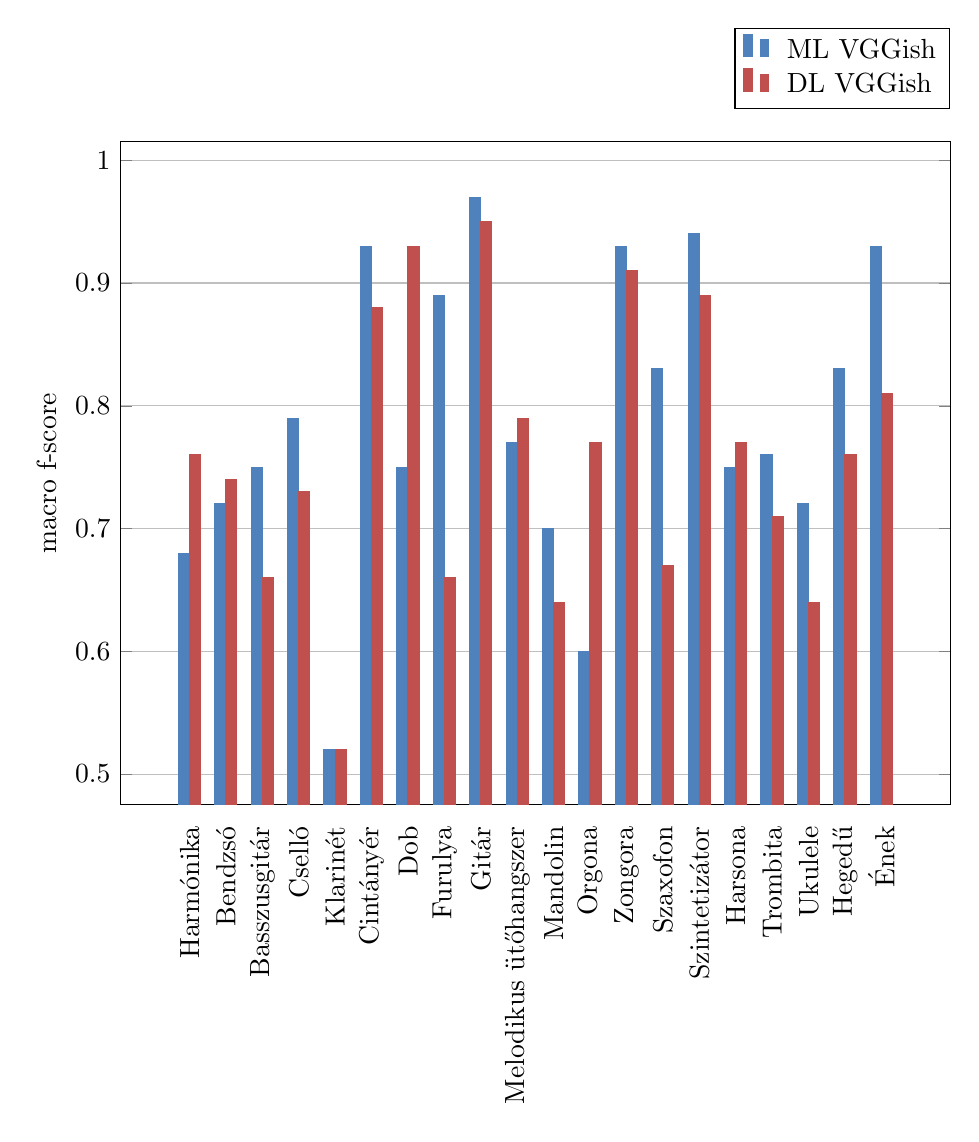
\begin{tikzpicture}
    \begin{axis}[
        width  = \textwidth,
        height = 10cm,
        major x tick style = transparent,
        ybar=0pt,
        bar width=4pt,
        ymajorgrids = true,
        ylabel = {macro f-score},
        symbolic x coords={Harmónika,Bendzsó,Basszusgitár,Cselló,Klarinét,Cintányér,Dob,Furulya,Gitár,Melodikus ütőhangszer,Mandolin,Orgona,Zongora,Szaxofon,Szintetizátor,Harsona,Trombita,Ukulele,Hegedű,Ének},
        xtick = data,
        x tick label style={rotate=90},
        scaled y ticks = false,
        legend cell align=left,legend style={
                at={(1,1.05)},
                anchor=south east,
                column sep=1ex}
    ]
        \addplot[style={bblue,fill=bblue,mark=none}]
            coordinates {(Harmónika, 0.68) (Bendzsó,0.72) (Basszusgitár,0.75)  (Cselló,0.79)  (Klarinét,0.52)  (Cintányér,0.93)  (Dob,0.75)  (Furulya,0.89)  (Gitár,0.97)  (Melodikus ütőhangszer,0.77)  (Mandolin,0.70)  (Orgona,0.60) (Zongora,0.93) (Szaxofon,0.83) (Szintetizátor,0.94) (Harsona,0.75) (Trombita,0.76) (Ukulele,0.72) (Hegedű,0.83) (Ének,0.93)};
        \addplot[style={rred,fill=rred,mark=none}]
            coordinates {(Harmónika, 0.76) (Bendzsó,0.74) (Basszusgitár,0.66) (Cselló,0.73) (Klarinét,0.52)  (Cintányér,0.88) (Dob,0.93) (Furulya,0.66) (Gitár,0.95)  (Melodikus ütőhangszer,0.79)  (Mandolin,0.64)  (Orgona,0.77) (Zongora,0.91) (Szaxofon,0.67) (Szintetizátor,0.89) (Harsona,0.77) (Trombita,0.71) (Ukulele,0.64) (Hegedű,0.76) (Ének,0.81)};
        \legend{ML VGGish ,DL VGGish}
    \end{axis}
\end{tikzpicture}
\caption{Modeling Baseline és Shallow CNN elődjének kezdeti értékei optimalizációk nélkül VGGish reprezentáción} \label{fig:vggishbase}
\end{figure}


\subsection{Alternatív reprezentációk}

//TODO MELSPEC, MFCC bevezetése, miért alacsonyabbak a számok, ml vs dl

\begin{figure}
\centering
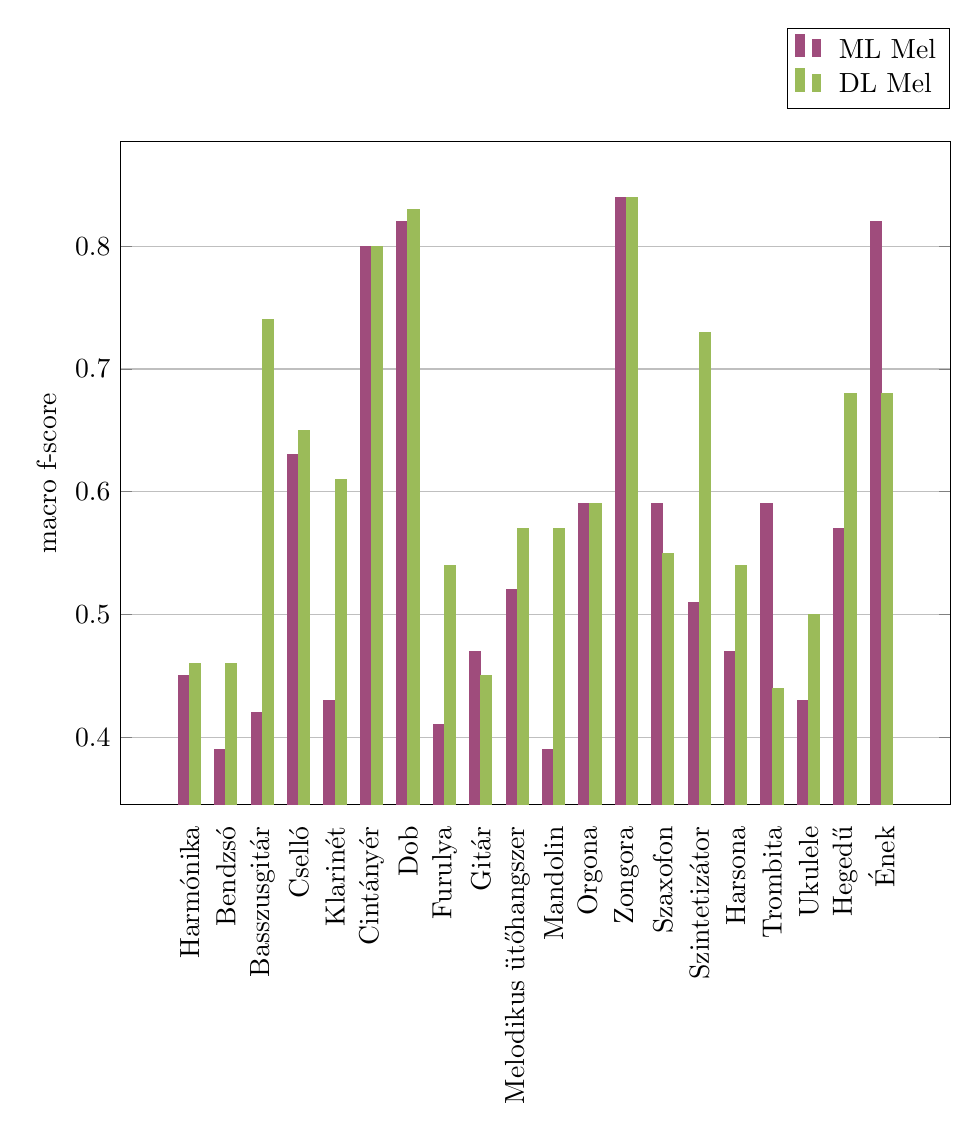
\begin{tikzpicture}
    \begin{axis}[
        width  = \textwidth,
        height = 10cm,
        major x tick style = transparent,
        ybar=0pt,
        bar width=4pt,
        ymajorgrids = true,
        ylabel = {macro f-score},
        symbolic x coords={Harmónika,Bendzsó,Basszusgitár,Cselló,Klarinét,Cintányér,Dob,Furulya,Gitár,Melodikus ütőhangszer,Mandolin,Orgona,Zongora,Szaxofon,Szintetizátor,Harsona,Trombita,Ukulele,Hegedű,Ének},
        xtick = data,
        x tick label style={rotate=90},
        scaled y ticks = false,
legend cell align=left,legend style={
                at={(1,1.05)},
                anchor=south east,
                column sep=1ex
        }
    ]
        \addplot[style={ppurple,fill=ppurple,mark=none}]
            coordinates {(Harmónika,0.45) (Bendzsó,0.39) (Basszusgitár,0.42) (Cselló,0.63)  (Klarinét,0.43)  (Cintányér,0.80)  (Dob,0.82)  (Furulya,0.41)  (Gitár,0.47)  (Melodikus ütőhangszer,0.52)  (Mandolin,0.39)  (Orgona,0.59) (Zongora,0.84) (Szaxofon,0.59) (Szintetizátor,0.51) (Harsona,0.47) (Trombita,0.59) (Ukulele,0.43) (Hegedű,0.57) (Ének,0.82) };

        \addplot[style={ggreen,fill=ggreen,mark=none}]
            coordinates {(Harmónika,0.46) (Bendzsó,0.46) (Basszusgitár,0.74) (Cselló,0.65)  (Klarinét,0.61)  (Cintányér,0.80)  (Dob,0.83)  (Furulya,0.54)  (Gitár,0.45)  (Melodikus ütőhangszer,0.57)  (Mandolin,0.57)  (Orgona,0.59) (Zongora,0.84) (Szaxofon,0.55) (Szintetizátor,0.73) (Harsona,0.54) (Trombita,0.44) (Ukulele,0.50) (Hegedű,0.68) (Ének,0.68) };
 	
        \legend{ML Mel,DL Mel}
    \end{axis}
\end{tikzpicture}
\caption{Modeling Baseline és Shallow CNN elődjének kezdeti értékei optimalizációk nélkül melspectogram reprezentáción} \label{fig:vggishbase}
\end{figure}
\cleardoublepage

\chapter{Összegzés, kitekintés}
\label{ch:sum}

A dolgozatom keretein belül megvizsgáltam a zenei információk kinyerése (MIR) tudományterület feladatait, megismerkedtem az automatikus hangszerfelismerés problémájával, ennek megközelítéseivel. Felkutattam különböző gépi tanulási és mély tanulási megoldásokat, tanító adathalmazokat.

Bemutattam egy CNN architektúrát, amellyel három különböző bemeneti reprezentáción kísérleteztem. A kísérletek konklúziójaként az látszik, hogy míg a bemutatott mély tanulási architektúra a már előre tanított, kisebb dimenziójú reprezentáción nagyjából egyforma teljesítményt nyújt, addig a nagyobb felbontású reprezentációkon már jobban teljesít, mint egy hagyományos gép tanulási megoldás.

A jövőben több módon is tovább lehetne optimalizálni a bemutatott modellt. A tapasztalataim alapján úgy gondolom, hogy a legnagyobb javulást az adathalmaz bővítése eredményezné. Erre azonban nem biztos, hogy van lehetőség, így én a következő továbbfejlesztéseket fontolnám meg:
\begin{itemize}
 \item Undersampling helyett oversampling, vagy data augmentation technikát alkalmazni az adatok előfeldolgozásakor
 \item A jelenlegi CNN architektúrát tovább mélyíteni, vagy helyette RNN architektúrát implementálni
 \item Az early stopping technika mellé model checkpointokat is bevezetni.
\end{itemize}

A felsoroltakon felül pedig érdemes lehet a melspectogram, MFCC és esetleg további reprezentációk mély tanulásra vonatkozó hatékonyságbeli különbségeit is tovább elemezni.
\cleardoublepage

% Irodalomjegyzék (kötelező)
% Bibliography (mandatory)
\addcontentsline{toc}{chapter}{\biblabel}
\printbibliography[title=\biblabel]
\cleardoublepage


\end{document}
